\documentclass{article}

\usepackage{tikz}
\usepackage[inner=0.5cm,outer=0.5cm]{geometry}

\begin{document}

\section*{Octahedron mmm}

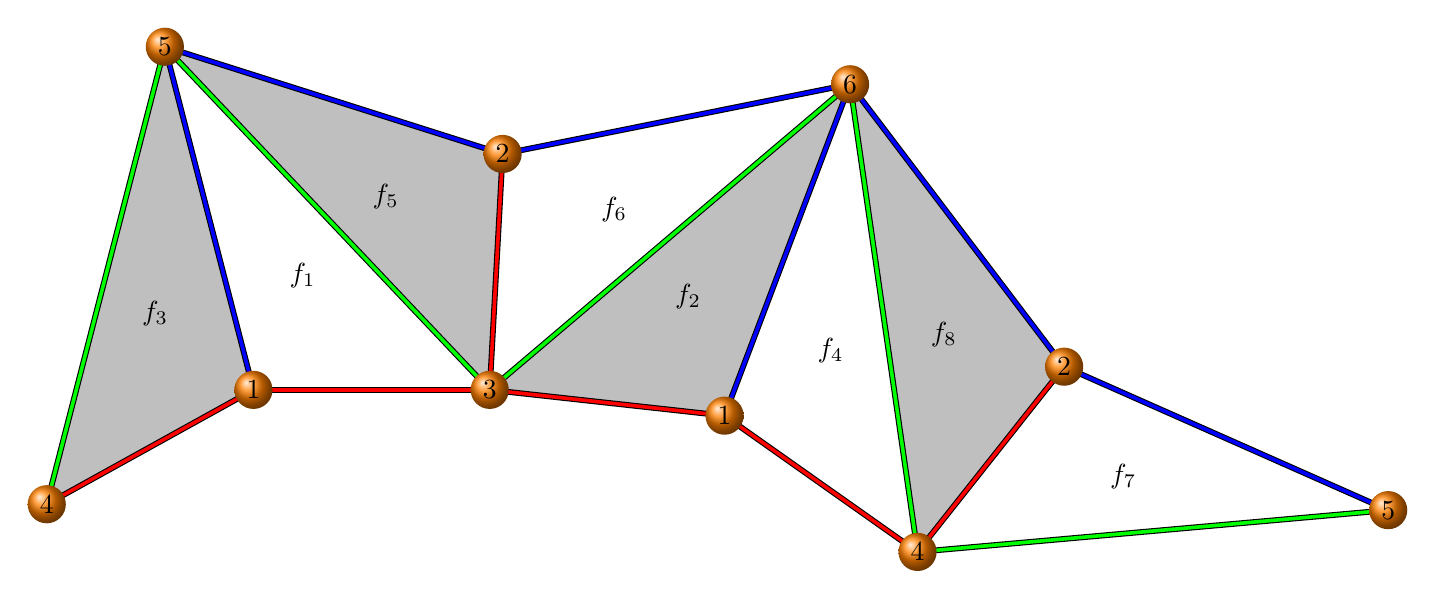
\begin{tikzpicture}[scale=3/2]
\coordinate (V1_1) at (0, 0);
\coordinate (V1_2) at (3.988037109375, -0.2184226447690221);
\coordinate (V2_1) at (2.109375, 1.997007037888199);
\coordinate (V2_2) at (6.863021850585938, 0.1962612562981385);
\coordinate (V3_1) at (2, 0);
\coordinate (V4_1) at (-1.75, -0.9682458365518543);
\coordinate (V4_2) at (5.621826171875, -1.371996785973379);
\coordinate (V5_1) at (-0.75, 2.904737509655563);
\coordinate (V5_2) at (9.606159210205078, -1.01831580023707);
\coordinate (V6_1) at (5.05078125, 2.587031844536985);


\fill[white] (V1_1) -- (V3_1) -- (V5_1) -- cycle;
\node (F1) at (0.4166666666666666, 0.9682458365518543) {$f_{1}$};
\fill[lightgray] (V1_2) -- (V3_1) -- (V6_1) -- cycle;
\node (F2) at (3.679606119791667, 0.7895363999226543) {$f_{2}$};
\fill[lightgray] (V1_1) -- (V4_1) -- (V5_1) -- cycle;
\node (F3) at (-0.8333333333333333, 0.6454972243679029) {$f_{3}$};
\fill[white] (V1_2) -- (V4_2) -- (V6_1) -- cycle;
\node (F4) at (4.886881510416666, 0.3322041379315279) {$f_{4}$};
\fill[lightgray] (V2_1) -- (V3_1) -- (V5_1) -- cycle;
\node (F5) at (1.119791666666667, 1.633914849181254) {$f_{5}$};
\fill[white] (V2_1) -- (V3_1) -- (V6_1) -- cycle;
\node (F6) at (3.053385416666667, 1.528012960808395) {$f_{6}$};
\fill[white] (V2_2) -- (V4_2) -- (V5_2) -- cycle;
\node (F7) at (7.363669077555338, -0.7313504433041036) {$f_{7}$};
\fill[lightgray] (V2_2) -- (V4_2) -- (V6_1) -- cycle;
\node (F8) at (5.845209757486979, 0.4704321049539147) {$f_{8}$};


\tikzset{EdgeStyle/.style = {thin, double distance=1.3pt} }

\draw[ EdgeStyle, double=red] (V3_1) -- (V1_1);
\draw[ EdgeStyle, double=red] (V1_2) -- (V3_1);
\draw[ EdgeStyle, double=red] (V1_1) -- (V4_1);
\draw[ EdgeStyle, double=red] (V4_2) -- (V1_2);
\draw[ EdgeStyle, double=blue] (V1_1) -- (V5_1);
\draw[ EdgeStyle, double=blue] (V6_1) -- (V1_2);
\draw[ EdgeStyle, double=red] (V2_1) -- (V3_1);
\draw[ EdgeStyle, double=red] (V2_2) -- (V4_2);
\draw[ EdgeStyle, double=blue] (V5_1) -- (V2_1);
\draw[ EdgeStyle, double=blue] (V2_2) -- (V5_2);
\draw[ EdgeStyle, double=blue] (V2_1) -- (V6_1);
\draw[ EdgeStyle, double=blue] (V6_1) -- (V2_2);
\draw[ EdgeStyle, double=green] (V5_1) -- (V3_1);
\draw[ EdgeStyle, double=green] (V6_1) -- (V3_1);
\draw[ EdgeStyle, double=green] (V4_1) -- (V5_1);
\draw[ EdgeStyle, double=green] (V5_2) -- (V4_2);
\draw[ EdgeStyle, double=green] (V6_1) -- (V4_2);



\tikzset{VertexStyle/.style = {
 shape = circle,
 ball color = orange,
 text = black,
 inner sep = 2pt,
 outer sep = 0pt,
 minimum size = 10pt} }

\node[VertexStyle] at (V1_1) {1};
\node[VertexStyle] at (V1_2) {1};
\node[VertexStyle] at (V2_1) {2};
\node[VertexStyle] at (V2_2) {2};
\node[VertexStyle] at (V3_1) {3};
\node[VertexStyle] at (V4_1) {4};
\node[VertexStyle] at (V4_2) {4};
\node[VertexStyle] at (V5_1) {5};
\node[VertexStyle] at (V5_2) {5};
\node[VertexStyle] at (V6_1) {6};

\end{tikzpicture}

\end{document} 
